\section{Phản ứng hạt nhân}
\subsection{Tóm tắt lí thuyết}
\begin{tomtat}
	\subsubsection{Phản ứng hạt nhân}
	\paragraph{Khái niệm}
	\begin{dn}
		Phản ứng hạt nhân là mọi quá trình dẫn đến sự biến đổi hạt nhân.\\
		Phản ứng hạt nhân được phân thành 2 loại:
		\begin{itemize}
			\item Phản ứng hạt nhân tự phát: hạt nhân kém bền vững tự phân rã thành các hạt nhân khác bền vững hơn.
			\item Phản ứng hạt nhân kích thích: trong đó các hạt nhân tương tác với nhau chủ yếu thông qua quá trình va chạm và biến đổi tạo thành các hạt nhân mới.
		\end{itemize}
	\end{dn}
	\paragraph{Phương trình tổng quát}
	\begin{equation}
		\ce{^{A_1}_{Z_1}X}+\ce{^{A_2}_{Z_2}Y\longrightarrow \ce{^{A_3}_{Z_3}C}}+\ce{^{A_4}_{Z_4}D}
	\end{equation}
	Trong đó, $\ce{X}$ và $\ce{Y}$ là các hạt nhân tương tác, $C$ và $D$ là các hạt sản phẩm.
	\subsubsection{Các định luật bảo toàn trong phản ứng hạt nhân}
	\paragraph{Bảo toàn số nucleon (số khối)}
	\begin{boxdl}
		Tổng số nucleon (số khối) của các hạt tương tác bằng tổng số nucleon (số khối) của các hạt sản phẩm:
		\begin{equation}
			A_1+A_2=A_3+A_4.
		\end{equation}
	\end{boxdl}
	\paragraph{Bảo toàn điện tích}
	\begin{boxdl}
		Tổng đại số điện tích của các hạt tương tác bằng tổng đại số điện tích của các hạt sản phẩm:
		\begin{equation}
			Z_1+Z_2=Z_3+Z_4.
		\end{equation}
	\end{boxdl}
	\paragraph{Bảo toàn động lượng}
\begin{boxdl}
		Vector tổng động lượng của các hạt tương tác bằng vector tổng động lượng của các hạt sản phẩm:
	\begin{equation}
		\vec{p}_{\ce{X}}+\vec{p}_{\ce{Y}}=\vec{p}_{\ce{C}}+\vec{p}_{\ce{D}}.
	\end{equation}
\end{boxdl}
	\paragraph{Bảo toàn năng lượng toàn phần}
	\begin{boxdl}
		Tổng năng lượng toàn phần (gồm năng lượng nghỉ và động năng) của các hạt tham gia phản ứng bằng tổng năng lượng toàn phần các hạt sản phẩm:
		\begin{equation}
			K_{\ce{X}}+m_{\ce{0X}}c^2+K_{\ce{Y}}+m_{\ce{0Y}}c^2=K_{\ce{C}}+m_{\ce{0C}}c^2+K_{\ce{D}}+m_{\ce{0D}}c^2.
		\end{equation}
	\end{boxdl}
	Trong đó, $K$ và $m_0c^2$ lần lượt là động năng và năng lượng nghỉ của các hạt.
\begin{note}
	Trong phản ứng hạt nhân không có định luật bảo toàn khối lượng.
\end{note}
\end{tomtat}
\subsection{Ví dụ minh hoạ}
\begin{dang}{Viết được đúng phương trình phân rã hạt nhân đơn giản}
Từ phương trình phản ứng hạt nhân: $\ce{^{A_1}_{Z_1}A}+\ce{^{A_2}_{Z_2}B}\longrightarrow\ce{^{A_3}_{Z_3}C}+\ce{^{A_4}_{Z_4}X}$, đề bài yêu cầu hãy xác định hạt nhân $\ce{X}$.
		\begin{itemize}
			\item Định luật bảo toàn số khối: $A_1+A_2=A_3+A_4\Rightarrow A_4$;
			\item Định luật bảo toàn điện tích: $Z_1+Z_2=Z_3+Z_4\Rightarrow Z_4$.
		\end{itemize}
\end{dang}
\begin{vd}
Cho phản ứng hạt nhân: $\ce{^4_2He}+\ce{^{14}_7N}\longrightarrow\ce{^1_1p}+\ce{X}$. Hãy xác định hạt nhân $\ce{X}$.
\loigiai{
Phương trình phản ứng hạt nhân:
$$\ce{^4_2He}+\ce{^{14}_7N}\longrightarrow\ce{^1_1p}+\ce{^A_ZX}.$$
Từ định luật bảo toàn số khối và điện tích, ta có:
\begin{align*}
	\begin{cases}
		4+14=1+A\\
		2+7=1+Z
	\end{cases}\Rightarrow\begin{cases}
		A=17\\
		Z=8
	\end{cases}
\end{align*}
}
\end{vd}
% =======================================
\begin{vd}
Bắn hạt $\alpha \left(\ce{^4_2He}\right)$ vào hạt nhân $\ce{^{27}_{13}Al}$ đứng yên, phản ứng sinh ra một hạt neutron và hạt nhân $\ce{X}$. So sánh số neutron $\left(\ce{^1_0n}\right)$ của hạt nhân $\ce{X}$ và hạt $\ce{^{27}_{13}Al}$.
\loigiai{
Phương trình phản ứng hạt nhân:
$$\ce{^4_2He}+\ce{^{27}_{13}Al}\longrightarrow\ce{^1_0n}+\ce{^A_ZX}.$$
Từ định luật bảo toàn số khối và bảo toàn điện tích, ta có:
\begin{align*}
	\begin{cases}
		4+27=1+A\\
		2+13=0+Z
	\end{cases}\Rightarrow\begin{cases}
		A=30\\
		Z=15
	\end{cases}
\end{align*}
Số neutron của hạt nhân $\ce{X}$ là 15; số neutron của hạt nhân $\ce{^{27}_{13}Al}$ là 14.\\
$\Rightarrow$ Số neutron của hạt nhân $\ce{X}$ nhiều hơn 1 hạt so với số neutron của hạt nhân $\ce{^{27}_{13}Al}$.
}
\end{vd}
\begin{dang}{Xác định được năng lượng của phản ứng hạt nhân}
		Năng lượng của phản ứng hạt nhân:
		\begin{equation}
			\Delta E=\left(m_\text{tt}-m_\text{sp}\right)c^2
		\end{equation}
		Trong đó:
		\begin{itemize}
			\item $m_\text{tt}=m_{0\ce{X}}+m_{0\ce{Y}}$: tổng khối lượng nghỉ của các hạt tương tác (trước phản ứng);
			\item $m_\text{sp}=m_{0\ce{C}}+m_{0\ce{D}}$: tổng khối lượng các hạt sản phẩm (sau phản ứng).
		\end{itemize}
		Khi đó:
		\begin{itemize}
			\item Trường hợp $m_\text{tt}>m_\text{sp}$ hay $\Delta E>0$: Phản ứng hạt nhân toả năng lượng;
			\item Trường hợp $m_\text{tt}<m_\text{sp}$ hay $\Delta E<0$: Phản ứng hạt nhân thu năng lượng.
		\end{itemize}
		Ngoài ra, năng lượng phản ứng hạt nhân còn được tính:
		$$\Delta E=\left(\Delta m_\text{sp}-\Delta m_\text{tt}\right)c^2=K_\text{sp}-K_\text{tt}.$$
		Với $\Delta m_\text{tt}$, $K_\text{tt}$; $\Delta m_\text{sp}$, $K_\text{sp}$ lần lượt là độ hụt khối, động năng của các hạt tương tác và các hạt sản phẩm.
\end{dang}
\begin{vd}
	Trong một phản ứng hạt nhân, tổng khối lượng nghỉ của các hạt tương tác là $\SI{37.9638}{u}$ và tổng khối lượng nghỉ của các hạt sản phẩm là $\SI{37.9656}{u}$. Lấy $\SI{1}{u}=\SI{931.5}{\mega\electronvolt/c^2}$. Phản ứng này thu hay toả một lượng năng lượng bằng bao nhiêu?
	\loigiai{
	Năng lượng của phản ứng hạt nhân:
	$$\Delta E=\left(m_\text{tt}-m_\text{sp}\right)c^2=\xsi{\left(37,9638-37,9656\right)}{uc^2}=\SI{-1.8E-3}{}\cdot\SI{931.5}{\mega\electronvolt}=\SI{-1.6767}{\mega\electronvolt}.$$
	Vậy phản ứng này thu năng lượng $\SI{1.6767}{\mega\electronvolt}$.	
	}
\end{vd}
% ===================================
\begin{vd}
	Xét phản ứng hạt nhân: $\ce{^2_1D}+\ce{^2_1D}\longrightarrow\ce{^4_2He}$. Biết độ hụt khối của $\ce{D}$ là $\SI{0.0024}{u}$; độ hụt khối của $\ce{He}$ là $\SI{0.0305}{u}$ và $\SI{1}{u}=\SI{931.5}{\mega\electronvolt/c^2}$. Phản ứng này toả hay thu một lượng năng lượng bằng bao nhiêu?
	\loigiai{
	Năng lượng phản ứng hạt nhân:
	$$\Delta E=\left(\Delta m_{\ce{He}}-2\Delta m_{\ce{D}}\right)c^2=\xsi{\left(0,0305-2\cdot0,0024\right)}{uc^2}=0,0257\cdot\SI{931.5}{\mega\electronvolt}=\SI{23.94}{\mega\electronvolt}.$$
	Vậy phản ứng này toả năng lượng $\SI{23.94}{\mega\electronvolt}$.
	}
\end{vd}
% =============================================
\begin{vd}
	Cho phản ứng hạt nhân: $\ce{^1_0n}+\ce{^{235}_{92}U}\longrightarrow \ce{^{94}_{38}Sr}+\ce{^{140}_{54}Xe}+2\ce{^1_0n}$. Biết năng lượng liên kết riêng của các hạt $\ce{U}$, $\ce{Sr}$ và $\ce{Xe}$ lần lượt là $\SI{7.59}{\mega\electronvolt/nucleon}$, $\SI{8.59}{\mega\electronvolt/nucleon}$ và $\SI{8.29}{\mega\electronvolt/nucleon}$. Năng lượng toả ra của phản ứng trên bằng bao nhiêu?
	\loigiai{
	Năng lượng của phản ứng hạt nhân:
	$$\Delta E=E_{\text{lk}\ce{Sr}}+E_{\text{lk}\ce{Xe}}-E_{\text{lk}\ce{U}}$$
	$$\Rightarrow \Delta E=94\cdot\left(\SI{8.59}{\mega\electronvolt}\right)+140\cdot\left(\SI{8.29}{\mega\electronvolt}\right)-235\cdot\left(\SI{7.59}{\mega\electronvolt}\right)=\SI{184.41}{\mega\electronvolt}.$$
	Vậy phản ứng này toả năng lượng $\SI{184.41}{\mega\electronvolt}$.
	
	}
\end{vd}
\begin{dang}{Vận dụng được định luật bảo toàn năng lượng toàn phần trong phản ứng hạt nhân}
	\end{dang}
\begin{vd}
Cho hạt proton có động năng $\SI{1.1}{\mega\electronvolt}$ bắn vào hạt nhân $\ce{^7_3Li}$ đứng yên, sau phản ứng thu được 2 hạt nhân $\ce{X}$ giống nhau. Giả thiết hai hạt sinh ra có cùng động năng. Cho khối lượng nghỉ của các hạt tương ứng là $m_p=\SI{1.0073}{u}$; $m_{\ce{Li}}=\SI{7.016}{u}$; $m_{\ce{X}}=\SI{4.0015}{u}$; $\SI{1}{u}=\SI{931.5}{\mega\electronvolt/c^2}$. Tính động năng của mỗi hạt $\ce{X}$ sinh ra.
\loigiai{Phương trình phản ứng hạt nhân:
	$$\ce{^1_1p}+\ce{^7_3Li}\longrightarrow2\ce{^4_2He}.$$
	Áp dụng định luật bảo toàn năng lượng toàn phần:
	$$m_pc^2+K_p+m_{\ce{Li}}c^2+K_{\ce{Li}}=2K_{\ce{X}}+2m_{\ce{X}}c^2$$
	$$\Rightarrow K_X=\dfrac{K_p+\left(m_p+m_{\ce{Li}}-2m_{\ce{X}}\right)c^2}{2}=\dfrac{\SI{1.1}{\mega\electronvolt}+0,0203\cdot\left(\SI{931.5}{\mega\electronvolt}\right)}{2}\approx\SI{10}{\mega\electronvolt}.$$}
\end{vd}
% =======================================
\begin{vd}
Bắn hạt $\ce{^4_2He}$ có động năng $\SI{4}{\mega\electronvolt}$ vào hạt $\ce{^{14}_7N}$ đang đứng yên thì thu được hạt proton và hạt nhân $\ce{X}$. Giả thiết các hạt sinh ra có cùng tốc độ. Cho khối lượng của các hạt lần lượt là $m_{\ce{He}}=\SI{4.0015}{u}$; $m_{\ce{X}}=\SI{16.9947}{u}$; $m_{\ce{N}}=\SI{13.9992}{u}$; $m_p=\SI{1.0073}{u}$; $\SI{1}{u}=\SI{931.5}{\mega\electronvolt/c^2}$. Động năng hạt proton bay ra bằng bao nhiêu?
\loigiai{Phương trình phản ứng:
	$$\ce{^4_2He}+\ce{^{14}_7N}\longrightarrow \ce{^1_1p}+X.$$
	Áp dụng định luật bảo toàn năng lượng toàn phần:
	$$m_{\ce{He}}c^2+K_{\ce{He}}+m_{\ce{N}}c^2=K_p+m_pc^2+K_{\ce{X}}+m_{\ce{X}}c^2$$
	\begin{equation}
		\label{eq:1}\\
		K_p+K_{\ce{X}}=K_{\ce{He}}+\left(m_{\ce{He}}+m_{\ce{N}}-m_p-m_{\ce{X}}\right)c^2=\SI{2.78905}{\mega\electronvolt}.
	\end{equation}	
	Vì hai hạt sản phẩm có cùng tốc độ nên:
	\begin{equation}
		\label{eq:2}\\
		\dfrac{K_p}{K_{\ce{X}}}=\dfrac{m_p}{m_{\ce{X}}}=0,0593.
	\end{equation}
	Từ \eqref{eq:1} và \eqref{eq:2}, ta có:
	\begin{align*}
		\begin{cases}
			K_p=\SI{0.156}{\mega\electronvolt}\\
			K_{\ce{X}}=\SI{2.633}{\mega\electronvolt}
		\end{cases}.
\end{align*}}
\end{vd}
\begin{dang}{Vận dụng định luật bảo toàn động lượng trong phản ứng hạt nhân}
	Ta có thể thu được phương trình liên hệ động năng các hạt trong phản ứng bằng cách bình phương hai vế phương trình bảo toàn động lượng:
	\begin{eqnarray*}
		&&\vec{p}_{\ce{A}}=\vec{p}_{\ce{B}}+\vec{p}_{\ce{C}}\\
		&\Rightarrow& p^2_{\ce{A}}=p^2_{\ce{B}}+p^2_{\ce{C}}+2\vec{p}_{\ce{B}}\vec{p}_{\ce{C}}=p^2_{\ce{B}}+p^2_{\ce{C}}+2p_{\ce{B}}p_{\ce{C}}\cos\left(\vec{p}_{\ce{B}},\vec{p}_{\ce{C}}\right)\\
	\end{eqnarray*}	
	Với $p^2=2mK$ thì
	$$m_{\ce{A}}K_{\ce{A}}=m_{\ce{B}}K_{\ce{B}}+m_{\ce{C}}K_{\ce{C}}+2\sqrt{m_{\ce{B}}K_{\ce{B}}m_{\ce{C}}K_{\ce{C}}}\cos\left(\vec{p}_{\ce{B}},\vec{p}_{\ce{C}}\right).$$
	\end{dang}
\begin{vd}
	Hạt nhân radium $\ce{^{226}_{88}Ra}$ đứng yên tự phân rã thành hạt $\alpha \left(\ce{^4_2He}\right)$ và hạt nhân radon $\ce{^{222}_{86}Rn}$. Biết khối lượng các hạt lần lượt là $m_{\ce{Ra}}=\SI{225.977}{u}$; $m_\alpha=\SI{4.0015}{u}$; $m_{\ce{Rn}}=\SI{221.970}{u}$; $\SI{1}{u}=\SI{931.5}{\mega\electronvolt/c^2}$. Động năng hạt $\alpha$ bằng bao nhiêu?
	\loigiai{
	Phương trình phản ứng hạt nhân:
	$$\ce{^{226}_{88}Ra}\longrightarrow\ce{^4_2He}+\ce{^{222}_{86}Rn}.$$
	Áp dụng định luật bảo toàn năng lượng toàn phần:
	$$m_{\ce{Ra}}c^2+K_{\ce{Ra}}=m_{\alpha}c^2+K_{\alpha}	+m_{\ce{Rn}}c^2+K_{\ce{Rn}}$$
	\begin{equation}
		\label{eq:3}\\
		K_{\alpha}+K_{\ce{Rn}}=\left(m_{\ce{Ra}}-m_\alpha-m_{\ce{Rn}}\right)c^2=\SI{5.12325}{\mega\electronvolt}.
	\end{equation}
	Áp dụng định luật bảo toàn động lượng:
	$$\vec{p}_{\ce{Ra}}=\vec{p}_{\ce{Rn}}+\vec{p}_\alpha\Rightarrow \vec{p}_\alpha=-\vec{p}_{\ce{Rn}}$$
	\begin{equation}
		\label{eq:4}
		\Leftrightarrow p^2_\alpha=p^2_{\ce{Rn}}\Leftrightarrow m_\alpha K_\alpha-m_{\ce{Rn}}K_{\ce{Rn}}=0\Leftrightarrow 4,0015K_\alpha-221,97K_{\ce{Rn}}=0
	\end{equation}
	Từ \eqref{eq:3} và \eqref{eq:4}, ta thu được:
	\begin{align*}
		\begin{cases}
			K_\alpha=\SI{5.0325}{\mega\electronvolt}\\
			K_{\ce{Rn}}=\SI{0.091}{\mega\electronvolt}
		\end{cases}.
	\end{align*}
	}
\end{vd}
% ================================================
\begin{vd}
	Dùng hạt $\alpha \left(\ce{^4_2He}\right)$ có động năng $\SI{40.85}{\mega\electronvolt}$ bắn phá hạt nhân aluminium $\ce{^{27}_{13}Al}$ đang đứng yên gây ra phản ứng hạt nhân. Phản ứng này sinh ra một neutron và hạt nhân $\ce{X}$ bay theo hai phương vuông góc nhau. Cho $m_{\ce{X}}=\SI{29.9970}{u}$; $m_{\ce{n}}=\SI{1.0087}{u}$; $m_{\ce{Al}}=\SI{26.97}{u}$; $m_\alpha=\SI{4.0015}{u}$; $\SI{1}{u}=\SI{931.5}{\mega\electronvolt/c^2}$. Động năng của hạt neutron sinh ra bằng bao nhiêu?
	\loigiai{
	Phương trình phản ứng:
	$$\ce{^4_2He}+\ce{^{27}_{13}Al}\longrightarrow \ce{^1_0n}+\ce{^{30}_{15}X}.$$
	Áp dụng định luật bảo toàn năng lượng toàn phần:
	$$m_\alpha c^2+K_\alpha+m_{\ce{Al}}c^2+K_{\ce{Al}}=m_{\ce{n}}c^2+K_{\ce{n}}+m_{\ce{X}}c^2+K_{\ce{X}}$$
	\begin{equation}
		\label{eq:5}
		\Rightarrow K_{\ce{n}}+K_{\ce{X}}=K_\alpha+\left(m_\alpha+m_{\ce{Al}}-m_{\ce{n}}-m_{\ce{X}}\right)c^2=\SI{8.9927}{\mega\electronvolt}.
	\end{equation}	
	Áp dụng định luật bảo toàn động lượng:
	$$\vec{p}_{\ce{He}}=\vec{p}_{\ce{n}}+\vec{p}_{\ce{X}}$$
	Do $\vec{p}_{\ce{n}}\bot\vec{p}_{\ce{X}}$ nên:
	$$p^2_{\ce{He}}=p^2_{\ce{n}}+p^2_{\ce{X}}\Leftrightarrow m_{\ce{He}}K_{\ce{He}}=m_{\ce{n}}K_{\ce{n}}+m_{\ce{X}}K_{\ce{X}}$$
	\begin{equation}
		\label{eq:6}\\
		\Rightarrow 1,0087K_{\ce{n}}+29,997K_{\ce{X}}=4,0015\cdot\left(\SI{40.85}{\mega\electronvolt}\right)=\SI{163.46}{\mega\electronvolt}.
	\end{equation}
	Từ \eqref{eq:5} và \eqref{eq:6}, ta thu được:
	\begin{align*}
		\begin{cases}
			K_{\ce{n}}=\SI{3.667}{\mega\electronvolt}\\
			K_{\ce{X}}=\SI{5.326}{\mega\electronvolt}
		\end{cases}.
	\end{align*}
	}
\end{vd}
\subsection{Bài tập}
\subsubsection{Trắc nghiệm nhiều phương án lựa chọn}
\setcounter{ex}{0}
\Opensolutionfile{ans}[ans/VN12-Y24-PH-SYL-027P-TN]
% ===================================================================
\begin{ex}
	Cho phản ứng hạt nhân: $\ce{^{19}_9F}+\ce{^1_1H}\longleftrightarrow\ce{^{16}_8O}+X$. $X$ là hạt	
	\choice
	{\True alpha}
	{neutron}
	{deuteri}
	{proton}
	\loigiai{}
\end{ex}
% ===================================================================
\begin{ex}
	Trong phản ứng hạt nhân: $\ce{^7_3Li}+\ce{X}\longrightarrow2\ce{^4_2He}$. Hạt $\ce{X}$ là
	\choice
	{$\ce{^3_1H}$}
	{$\ce{^2_1H}$}
	{\True $\ce{^1_1H}$}
	{$\ce{^1_0n}$}
	\loigiai{}
\end{ex}
% ===================================================================
\begin{ex}
	Cho phản ứng hạt nhân sau: $\ce{_4^9Be}+\ce{^1_1p} \longrightarrow \ce{X}+\ce{_3^6Li}$. Hạt nhân $\ce{X}$ là
	\choice
	{\True helium $\left(\ce{^4_2He}\right)$}
	{proton $\left(\ce{^1_1p}\right)$}
	{tritium $\left(\ce{^3_1T}\right)$}
	{deuterium $\left(\ce{^2_1D}\right)$}
	\loigiai{}
\end{ex}
% ===================================================================
\begin{ex}
	Cho phản ứng hạt nhân sau: $\ce{_{17}^{37}Cl}+\ce{X} \longrightarrow \ce{_0^1n}+\ce{_{18}^{37}Ar}$. Biết điện tích nguyên tố là $e$. Điện tích của hạt nhân $\ce{X}$ là
	\choice
	{\True $+e$}
	{$0$}
	{$+2e$}
	{$+4e$}
	\loigiai{}
\end{ex}
% ===================================================================
\begin{ex}
	Trong phản ứng hạt nhân: $\ce{_4^9Be}+\ce{_2^4He} \longrightarrow \ce{_0^1n}+\ce{X}$, hạt nhân $\ce{X}$ có	
	\choice
	{\True 6 neutron và 6 proton}
	{6 nucleon và 6 proton}
	{12 neutron và 6 proton}
	{6 neutron và 12 proton}
	\loigiai{}
\end{ex}
% ===================================================================
\begin{ex}
	Xét phản ứng: $\ce{_{90}^{232}Th} \longrightarrow \ce{_{82}^{208}Pb}+x \ce{_2^4He}+y \ce{_{-1}^0\beta}$. Ti số $\dfrac{x}{y}$ bằng
	\choice
	{$\dfrac{x}{y}=\dfrac{2}{3}$}
	{\True $\dfrac{x}{y}=\dfrac{3}{2}$}
	{$\dfrac{x}{y}=\dfrac{1}{2}$}
	{$\dfrac{x}{y}=2$}
	\loigiai{
		Ta có: 
		$$\begin{cases}
			232=208+4x\\
			90=82+2x-y
		\end{cases}\Leftrightarrow\begin{cases}
			x=6\\
			y=4
		\end{cases}\Rightarrow\dfrac{x}{y}=\dfrac{3}{2}.$$
	}
\end{ex}
% ===================================================================
\begin{ex}
	Giả sử trong một phản ứng hạt nhân, tổng khối lượng của các hạt tương tác nhỏ hơn tổng khối lượng các hạt sản phẩm là $\SI{0.02}{u}$. Biết $\SI{1}{u}=\SI{931.5}{\mega\electronvolt/c^2}$. Phản ứng hạt nhân này	
	\choice
	{\True thu năng lượng $\SI{18.63}{\mega\electronvolt}$}
	{thu năng lượng $\SI{1.863}{\mega\electronvolt}$}
	{tỏa năng lượng $\SI{1.863}{\mega\electronvolt}$}
	{tỏa năng lượng $\SI{18.63}{\mega\electronvolt}$}
	\loigiai{
		$$E=\left(m_{\text{tt}}-m_{\text{sp}}\right)c^2=\SI{-18.63}{\mega\electronvolt}.$$
	}
\end{ex}

% ===================================================================
\begin{ex}
	Dùng một proton bắn phá hạt nhân sodium $\ce{_{11}^{23}Na}$ đứng yên sinh ra hạt $\alpha$ và hạt $X$. Coi phản ứng không kèm theo bức xạ $\gamma$. Cho $m_p=\SI{1.0073}{u}$; $m_{\ce{Na}}=\SI{22.9850}{u}$; $m_{\ce{X}}=\SI{=19.9869}{u}$; $m_\alpha=\SI{4.0015}{u}$; $\SI{1}{u}=\SI{931.5}{\mega\electronvolt/c^2}$. Phản ứng này	
	\choice
	{thu năng lượng $\Delta E=\SI{3.63}{\mega\electronvolt}$}
	{\True tỏa năng lượng $\Delta E=\SI{3.63}{\mega\electronvolt}$}
	{thu năng lượng $\Delta E=\SI{9.21}{\mega\electronvolt}$}
	{tỏa năng lượng $\Delta E=\SI{9.21}{\mega\electronvolt}$}
	\loigiai{
		$\Delta E=\left(m_p+m_{\ce{Na}}-m_\alpha-m_{\ce{X}}\right)c^2=\SI{3.63}{\mega\electronvolt}>0$.
	}
\end{ex}
% ===================================================================
\begin{ex}
	Dùng proton bắn vào hạt nhân $\ce{_3^7Li}$ thì thu được hai hạt nhân giống nhau $\ce{X}$. Biết độ hụt khối các hạt nhân $\ce{Li}$ và $\ce{X}$ lần lượt là $\Delta m_{\ce{Li}}=\SI{0.0427}{u}$; $\Delta m_{\ce{X}}=\SI{0.0305}{u}; 1 \ce{u}=931,5 \ce{MeV} / \ce{c}^2$. Phản ứng này thu hay tỏa bao nhiêu năng lượng?
	\choice
	{Tỏa ra $\SI{12.07}{\mega\electronvolt}$}
	{Thu $\SI{12.07}{\mega\electronvolt}$}
	{\True Tỏa ra $\SI{17.05}{\mega\electronvolt}$}
	{Thu $\SI{17.05}{\mega\electronvolt}$}
	\loigiai{
		$\Delta E=\left(2\Delta m_{\ce{X}}-\Delta m_{\ce{Li}}\right)c^2=\SI{17.05}{\mega\electronvolt}>0.$
	}
\end{ex}
% ===================================================================
\begin{ex}
	Xét phản ứng hạt nhân sau: 
	$$\ce{D}+\ce{T} \rightarrow \ce{He}+\ce{n}+\SI{18.1}{\mega\electronvolt}.$$
	Biết độ hụt khối các hạt nhân: $\ce{D}$; $\ce{T}$ lần lượt là $\Delta m_{\ce{D}}=\SI{0.0024}{u}$; $\Delta m_{\ce{T}}=\SI{0.0087}{u}$ và $\SI{1}{u}=\SI{931.5}{\mega\electronvolt/c^2}$. Độ hụt khối của hạt nhân He bằng
	\choice
	{\True $\SI{0.0305}{u}$}
	{$\SI{0.0111}{u}$}
	{$\SI{6.3E-3}{u}$}
	{$\SI{0.1140}{u}$}
	\loigiai{
		$\Delta E=\left(\Delta m_{\ce{He}}-\Delta m_{\ce{D}}-\Delta m_{\ce{T}}\right)c^2=\SI{18.1}{\mega\electronvolt}\Rightarrow \Delta m_{\ce{He}}\approx\SI{0.0305}{u}.$
	}
\end{ex}
% ===================================================================
\begin{ex}
	Cho phản ứng hạt nhân: $\ce{_{17}^{37}Cl}+p \longrightarrow n+ \ce{_{18}^{37}Ar}$. Khối lượng của các hạt là $m_{\ce{Cl}}=\SI{36.9566}{u}$; $m_p=\SI{1.0073}{u}$;   $m_n=\SI{1.0087}{u}$ và phản ứng thu một lượng năng lượng là $\SI{1.58}{\mega\electronvolt}$. Lấy $\SI{1}{u}=\SI{931.5}{\mega\electronvolt/c^2}$. Khối lượng của hạt nhân $\ce{Ar}$ bằng
	\choice
	{\True $\SI{36.9569}{u}$}
	{$\SI{37.0023}{u}$}
	{$\SI{36.9535}{u}$}
	{$\SI{37.2103}{u}$}
	\loigiai{
		$\Delta E=\left(m_{\ce{Cl}}+m_p-m_n-m_{\ce{Ar}}\right)c^2\Rightarrow m_{\ce{Ar}}\approx\SI{36.9569}{u}$.
	}
\end{ex}
% ===================================================================
\begin{ex}
	Đây là phản ứng phân hạch của một hạt $\ce{U^{235}}$:
	$$
	\ce{_{92}^{235}U}+\ce{_0^1n} \longrightarrow\ce{_{58}^{140}Ce}+ \ce{_{41}^{93}Nb}+3 \ce{_0^1n}+7 \ce{e}
	$$
	Biết năng lượng liên kết riêng của $\ce{_{92}^{235}U}$ là $\SI{7.7}{\mega\electronvolt/nucleon}$, của $\ce{_{58}^{140}Ce}$ là $\SI{8.43}{\mega\electronvolt/nucleon}$, của $\ce{_{41}^{93}Nb}$ là $\SI{8.7}{\mega\electronvolt/nucleon}$. Năng lượng toả ra của phản ứng là
	\choice
	{$\SI{187.4}{\mega\electronvolt}$}
	{$\SI{179.7}{\mega\electronvolt}$}
	{\True $\SI{179.8}{\mega\electronvolt}$}
	{$\SI{182.6}{\mega\electronvolt}$}
	\loigiai{
		$\Delta E=E_{\text{lk}\ce{Ce}}+E_{\text{lk}\ce{Nb}}-E_{\text{lk}\ce{U}}=140\cdot8,43+93\cdot 8,7-235\cdot 7,7=\SI{179.8}{\mega\electronvolt}.$
	}
\end{ex}
% ===================================================================
\begin{ex}
	Bắn một proton vào hạt nhân $\ce{^7_3Li}$ đứng yên. Phản ứng tạo ra hai hạt nhân $\ce{X}$ giống nhau bay ra với cùng tốc độ theo các phương hợp với phương tới của proton các góc bằng nhau là $\SI{60}{\degree}$. Lấy khối lượng của mỗi hạt nhân tính theo đơn vị $\si{u}$ bằng số khối của nó. Tỉ số giữa tốc độ của proton và tốc độ của hạt nhân $\ce{X}$ là
	\choice
	{\True 4}
	{$\dfrac{1}{4}$}
	{2}
	{$\dfrac{1}{2}$}
	\loigiai{
		Phương trình phản ứng: $\ce{^1_1p}+\ce{^7_3Li}\longrightarrow2\ce{^4_2X}$.\\
		Áp dụng định luật bảo toàn động lượng:
		$$\vec{p}_{\ce{p}}=\vec{p}_{\ce{X}}+\vec{p}_{\ce{X}}$$
		Do hai hạt nhân $\ce{X}$ giống nhau bay ra với cùng tốc độ theo các phương hợp với phương tới của proton các góc bằng nhau $\SI{60}{\degree}$ nên:
		\begin{eqnarray*}
			&&p^2_{\ce{p}}=p^2_{\ce{X}}+p^2_{\ce{X}}+2p_{\ce{X}}p_{\ce{X}}\cos
			\SI{120}{\degree}\\
			&\Rightarrow& p_{\ce{p}}=p_{\ce{X}}\\
			&\Leftrightarrow& m_{\ce{p}}v_{\ce{p}}=m_{\ce{X}}v_{\ce{X}}\\
			&\Rightarrow& \dfrac{v_{\ce{p}}}{v_{\ce{X}}}=\dfrac{m_{\ce{X}}}{m_{\ce{p}}}=4.
		\end{eqnarray*}
		
	}
\end{ex}
% ===================================================================
\begin{ex}
	Người ta dùng hạt $\alpha$ có động năng $K_{\alpha}$  bắn vào hạt nhân nhôm $\ce{^{27}_{13}Al}$  đứng yên gây ra phản ứng $\ce{^4_2He}+\ce{^{27}_{13}Al}\longrightarrow\ce{^{30}_{15}P}+\ce{^1_0n}$.  Biết hạt neutron và hạt nhân $\ce{^{30}_{15}P}$  sinh ra sau phản ứng có động năng lần lượt là $\SI{1.8}{\mega\electronvolt}$ và $\SI{1}{\mega\electronvolt}$. Biết khối lượng của các hạt lần lượt là $m_{\alpha}=\SI{4.00151}{u}$; $m_{\ce{Al}}=\SI{26.97435}{u}$; $m_{\ce{P}}=\SI{29.97005}{u}$; $m_{\ce{n}}=\SI{1.00867}{u}$. Động năng hạt $\alpha$ là 
	\choice
	{\True $\SI{5.464}{\mega\electronvolt}$}
	{$\SI{4.232}{\mega\electronvolt}$}
	{$\SI{5.644}{\mega\electronvolt}$}
	{$\SI{4.328}{\mega\electronvolt}$}
	\loigiai{
		Bảo toàn năng lượng toàn phần:
		$$\Delta E+K_{\alpha}+K_{\ce{Al}}=K_{\ce{P}}+K_{\ce{n}}$$
		$$\Leftrightarrow \left(m_{\alpha}+m_{\ce{Al}}-m_{\ce{P}}-m_{\ce{n}}\right)c^2+K_{\ce{Al}}=K_{\ce{P}}+K_{\ce{n}}$$
		$$\Rightarrow K_{\alpha}=\SI{5.464}{\mega\electronvolt}.$$
	}
\end{ex}
% ===================================================================
\begin{ex}
	Proton có động năng $K_{\ce{P}}=\SI{5.0}{\mega\electronvolt}$ được bắn vào $\ce{^9_4Be}$  nằm yên. Phản ứng hạt nhân sinh ra $\ce{^4_2He}$   và $\ce{X}$. Sau phản ứng hạt nhân $\ce{^4_2He}$  có động năng  $K_{\ce{He}}=\SI{4.1}{\mega\electronvolt}$ và vận tốc $\vec{v}_{\ce{He}}$   vuông góc với vận tốc $\vec{v}_{\ce{p}}$   lúc đầu. Động năng của hạt nhân $\ce{X}$ là
	\choice
	{$\SI{7.40}{\mega\electronvolt}$}
	{$\SI{9.10}{\mega\electronvolt}$}
	{\True $\SI{3.57}{\mega\electronvolt}$}
	{$\SI{0.90}{\mega\electronvolt}$}
	\loigiai{
		Phương trình phản ứng: $\ce{^1_1p}+\ce{^9_4Be}\longrightarrow\ce{^4_2He}+\ce{^6_3X}$.\\
		Áp dụng định luật bảo toàn động lượng:
		$$\vec{p}_{\ce{p}}=\vec{p}_{\ce{He}}+\vec{p}_{\ce{X}}$$
		Vì $\vec{p}_{\ce{He}}\bot\vec{p}_{\ce{p}}$ nên:
		$$p^2_{\ce{X}}=p^2_{\ce{p}}+p^2_{\ce{He}}\Leftrightarrow m_{\ce{X}}K_{\ce{X}}=m_{\ce{He}}K_{\ce{He}}+m_{\ce{p}}K_{\ce{p}}\Rightarrow K_{\ce{X}}=\SI{3.57}{\mega\electronvolt}.$$
	}
\end{ex}
% ===================================================================
\begin{ex}
	Người ta dùng proton có động năng $K_{\ce{p}}=\SI{5.45}{\mega\electronvolt}$   bắn phá vào bia beryllium, phản ứng xảy ra theo phương trình sau:
	$$\ce{^9_4Be}+\ce{p}\longrightarrow\ce{X}+\ce{^6_3Li}$$
	Biết khối lượng các hạt lần lượt là $m_{\ce{Be}}=\SI{9.01219}{u}$, $m_{\ce{p}}=\SI{1.00873}{u}$, $m_{\ce{X}}=\SI{4.00620}{u}$, $m_{\ce{Li}}=\SI{6.01515}{u}$, $\SI{1}{u}=\SI{931}{\mega\electronvolt/c^2}$ và hạt nhân lithium bay ra với động năng $\SI{3.55}{\mega\electronvolt}$. Động năng của hạt X bay ra có giá trị là
	
	\choice
	{$\SI{66}{\mega\electronvolt}$}
	{\True $\SI{0.66}{\mega\electronvolt}$}
	{$\SI{0.66}{\electronvolt}$}
	{$\SI{660}{\electronvolt}$}
	\loigiai{
		Bảo toàn năng lượng toàn phần:
		\begin{eqnarray*}
			&&\Delta E+K_{\ce{Be}}=K_{\ce{X}}+K_{\ce{Li}}\\
			&\Leftrightarrow& \left(m_{\ce{Be}}+m_{\ce{p}}-m_{\ce{X}}-m_{\ce{^6_3Li}}\right)c^2+K_{\ce{Be}}=K_{\ce{X}}+K_{\ce{Li}}\\
			&\Rightarrow& K_{\ce{X}}=\SI{0.66}{\mega\electronvolt}.
		\end{eqnarray*}
		
	}
\end{ex}
% ===================================================================
\begin{ex}
	Bắn hạt neutron có động năng $\SI{2}{\mega\electronvolt}$ vào hạt nhân $\ce{^6_3Li}$   đứng yên gây ra phản ứng $\ce{^1_0n}+\ce{^6_3Li}\longrightarrow\ce{X}+\alpha$. Hạt $\alpha$ và hạt nhân $\ce{X}$ bay ra theo các hướng hợp với hướng tới của neutron những góc tương ứng bằng $\theta=\SI{15}{\degree}$ và $\varphi=\SI{30}{\degree}$. Lấy tỉ số giữa các khối lượng hạt nhân bằng tỉ số giữa các số khối của chúng. Bỏ qua bức xạ gamma. Năng lượng của phản ứng hạt nhân trên là
	\choice
	{Tỏa $\SI{1.52}{\mega\electronvolt}$}
	{Thu $\SI{1.52}{\mega\electronvolt}$}
	{\True Thu $\SI{1.68}{\mega\electronvolt}$}
	{Tỏa $\SI{1.68}{\mega\electronvolt}$}
	\loigiai{
		Áp dụng định luật bảo toàn động lượng:
		$$\vec{p}_{\ce{n}}=\vec{p}_{\ce{X}}+p_{\ce{\alpha}}$$
		\begin{center}
			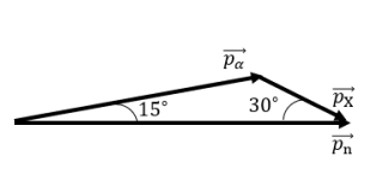
\includegraphics[width=0.4\linewidth]{figs/VN12-Y24-PH-SYL-029P-1}
		\end{center}
		Áp dụng định lý hàm sin trong tam giác động lượng:
		$$\dfrac{p_{\ce{n}}}{\sin\SI{135}{\degree}}=\dfrac{p_{\alpha}}{\sin\SI{30}{\degree}}\Rightarrow \dfrac{\sqrt{2m_{\ce{n}}K_{\ce{n}}}}{\sin\SI{135}{\degree}}=\dfrac{\sqrt{2m_{\alpha}K_{\alpha}}}{\sin\SI{30}{\degree}}\Rightarrow K_{\alpha}=\SI{0.25}{\mega\electronvolt}.$$
		Tương tự: $K_{\ce{X}}\approx\SI{0.089}{\mega\electronvolt}$.\\
		Năng lượng phản ứng:
		$$E=K_{\alpha}+K_{\ce{X}}-K_{n}=\SI{-1.66}{\mega\electronvolt}.$$
	}
\end{ex}
\Closesolutionfile{ans}
\subsubsection{Trắc nghiệm đúng/sai}
\setcounter{ex}{0}
\Opensolutionfile{ans}[ans/VN12-Y24-PH-SYL-027P-TF]
% ===================================================================
\begin{ex}
	Quá trình phản ứng hạt nhân.
	\choiceTF[t]
	{\True là quá trình biến đổi của các hạt nhân}
	{\True tuân theo định luật bảo toàn điện tích}
	{chỉ xảy ra quá trình tỏa năng lượng}
	{chỉ xảy ra khi có hai hạt nhân tương tác với nhau}
	\loigiai{
		\begin{itemchoice}
			\itemch Quá trình phản ứng hạt nhân là quá trình biến đổi của các hạt nhân.
			\itemch Trong phản ứng hạt nhân có sự bảo toàn về: số nucleon, điện tích, năng lượng toàn phần, động lượng.
			\itemch Phản ứng hạt nhân bao gồm phản ứng tỏa năng lượng và phản ứng thu năng lượng.
			\itemch Phản ứng hạt nhân là quá trình biến đổi từ hạt nhân này sang hạt nhân khác. Một số đồng vị không bền có thể tự phân rã để tạo thành hạt nhân khác.
		\end{itemchoice}
	}
\end{ex}
% ===================================================================
\begin{ex}
	Nhận định về các phát biểu sau đây.
	\choiceTFt
	{\True Phản ứng hạt nhân là quá trình biến đổi từ hạt nhân này thành hạt nhân khác, bao gồm phản ứng hạt nhân kích thích và phản ứng hạt nhân tự phát}
	{Trong một phản ứng hạt nhân, luôn cần từ hai hạt tham gia phản ứng trở lên}
	{\True Trong phản ứng hạt nhân, số khối và điện tích của hệ được	bảo toàn}
	{Trong phản ứng hạt nhân, số khối, điện tích và khối lượng của hệ được bảo toàn}
	{\True Phản ứng hạt nhân kích thích: là quá trình các hạt nhân tương tác với các hạt khác (ví dụ: hạt nhân, neutron,...) tạo ra các hạt nhân mới. Ví dụ: phản ứng phân hạch, phản ứng tổng hợp hạt nhân}
	{\True Phản ứng hạt nhân tự phát: là quá trình tự phân rã của một hạt nhân không bền vững thành các hạt nhân mới}
	\loigiai{}
\end{ex}
% ===================================================================
\begin{ex}
	Vào năm 1925, Patrick Blackett đã làm thí nghiệm bắn phá hạt alpha vào hạt nhân $\ce{^{14}_7N}$, tạo ra hai hạt nhân mới theo phương trình:
	$$\ce{^4_2He}+\ce{^{14}_7N}\longrightarrow\ce{^{17}_8O}+\ce{^1_1H}$$
	\choiceTF[t]
	{\True Đây là phản ứng hạt nhân kích thích}
	{Mỗi hạt nhân $\ce{^{17}_8O}$ có nhiều hơn hạt nhân $\ce{^{14}_7N}$ là 3 neutron}
	{\True $\ce{^{17}_8O}$ là một đồng vị của nguyên tố oxygen $\ce{^{16}_8O}$}
	{Trong phản ứng trên, điện tích và khối lượng nghỉ của các hạt nhân được bảo toàn}
	\loigiai{}
\end{ex}
% ===================================================================
\begin{ex}
	Hạt $\ce{^{210}_{84}Po}$ chuyển thành hạt $\ce{^{206}_{82}Pb}$ sau khi tự phóng ra hạt nhân $\ce{X}$. Biết đây là phản ứng hạt nhân tỏa năng lượng.
	\choiceTF[t]
	{Mối liên hệ khối lượng giữa các hạt là $m_{\ce{Po}}<m_{\ce{Pb}}+m_{\ce{X}}$}
	{Hạt nhân $\ce{X}$ là $\ce{^{12}_6C}$}
	{\True Điện tích của hạt $\ce{Po}$ bằng tổng điện tích của hạt $\ce{Pb}$ và hạt $\ce{X}$}
	{Mối liên hệ khối lượng giữa các hạt là $m_{\ce{Po}}=m_{\ce{Pb}}+m_{\ce{X}}$}
	\loigiai{
		\begin{itemchoice}
			\itemch Sai. Phản ứng tỏa năng lượng nên $m_{\ce{Po}}>m_{\ce{Pb}}+m_{\ce{X}}$.
			\itemch Sai. Hạt nhân $\ce{X}$ là $\ce{^4_2He}$.
			\itemch Đúng.
			\itemch Sai. Trong các phản ứng hạt nhân không có sự bảo toàn khối lượng.
		\end{itemchoice}
	}
\end{ex}
% ===================================================================
\begin{ex}
	Một phản ứng tổng hợp hạt nhân có phương trình: $\ce{_1^2D}+ \ce{_1^2D} \longrightarrow\ce{_1^3T}+\ce{X}$ Cho biết tổng khối lượng của các hạt trước phản ứng lớn hơn tổng khối lượng của các hạt sau phản ứng là $\SI{0.00432}{u}$. Các ý a ), b), c), d) dưới đây là đúng hay sai?
	\choiceTF[t]
	{\True Hạt nhân $X$ có điện tích $+1 e$}
	{\True Năng lượng toả ra của một phản ứng là $\SI{4.02}{\mega\electronvolt}$}
	{Năng lượng toả ra khi $\SI{1.00}{\gram}$ hạt nhân $\ce{_1^2D}$ được tổng hợp hoàn toàn là $\SI{2.0E11}{\joule}$}
	{Biết rằng nhiệt nóng chảy riêng của nước đá là $\SI{3.33E5}{\joule/\kilogram}$. Năng lượng toả ra khi tổng hợp hoàn toàn $\SI{1.00}{\gram}$ hạt nhân $\ce{_1^2D}$ có thể làm nóng chảy hoàn toàn $\SI{2.91E6}{\kilogram}$ nước đá ở $\SI{0}{\celsius}$}
	\loigiai{
		\begin{itemchoice}
			\itemch Đúng. $\ce{_1^2D}+\ce{_1^2D} \longrightarrow\ce{_1^3T}+\ce{_1^1H}$ nên hạt nhân X là $\ce{_1^1H}$.
			\itemch Đúng. $E_{\text {tỏa}}=\SI{4.02}{\mega\electronvolt}$.
			\itemch Sai. Mỗi phản ứng cần sử dụng 2 hạt nhân $\ce{_1^2D}$. Tổng năng lượng tỏa ra nếu tổng hợp hoàn toàn $\SI{1.00}{\gram}$ deterium là: $E=\SI{9.71E10}{\joule}$.
			\itemch Sai. $m=\dfrac{E}{\lambda}=\dfrac{\SI{9.71E10}{\joule}}{\SI{3.33E5}{\joule/\kilogram}}=\SI{2.92E5}{\kilogram}$.
		\end{itemchoice}
	}
\end{ex}
% ===================================================================
\begin{ex}
	Cho hạt $\alpha$  có động năng $K_{\alpha}$  bắn vào hạt nhân   đứng yên. Sau phản ứng sinh ra hạt nhân $\ce{^{30}_{15}P}$  và hạt neutron. Biết hạt nhân $\ce{^{30}_{15}P}$  và neutron có động năng lần lượt là $\SI{2.88E-13}{\joule}$  và $\SI{1.6E-13}{\joule}$. Cho khối lượng các hạt nhân là $m_{\ce{Al}}=\SI{26.9743}{u}$, $m_{\alpha}=\SI{4.0015}{u}$, $m_{\ce{P}}=\SI{29.9701}{u}$, $m_{\ce{n}}=\SI{1.0087}{u}$. Biết $\SI{1}{u}=\SI{931.5}{\mega\electronvolt/c^2}$.
	\choiceTF[t]
	{\True Phương trình phản ứng $\ce{^{27}_{13}Al}+\alpha\longrightarrow\ce{^{30}_{15}P}+\ce{n}$}
	{Phản ứng tỏa năng lượng}
	{\True Năng lượng phản ứng $\Delta E=\SI{2.7945}{\mega\electronvolt}$}
	{\True Động năng của hạt $\alpha$ là $K_{\alpha}=\SI{8.8E-16}{\joule}$}
	\loigiai{
		\begin{itemchoice}
			\itemch Phương trình phản ứng $\ce{^{27}_{13}Al}+\alpha\longrightarrow\ce{^{30}_{15}P}+\ce{n}$.
			\itemch Phản ứng có $m_{\text{trước}}>m_{\text{sau}}$ nên phản ứng thu năng lượng.
			\itemch Năng lượng phản ứng: $\Delta E=\left(m_{\text{trước}}-m_{\text{sau}}\right)c^2=\SI{2.7945}{\mega\electronvolt}$.
			\itemch Động năng của hạt $\alpha$:
			$$K_{\alpha}=K_{\ce{P}}+K_{\ce{n}}-\Delta E-K_{\ce{Al}}=\SI{5.5E-3}{\mega\electronvolt}\approx\SI{8.8E-16}{\joule}.$$
		\end{itemchoice}
	}
\end{ex}
\Closesolutionfile{ans}
\subsubsection{Tự luận}
\setcounter{ex}{0}
\Opensolutionfile{ans}[ans/VN12-Y24-PH-SYL-027P-TL]
% ======================================================================
\begin{ex}
	Cho phản ứng tổng hợp hạt nhân: $\ce{_3^6Li}+\ce{_1^2D} \longrightarrow\ce{_2^4He}+ \ce{^A_ZX}$ Biết khối lượng nguyên tử của các hạt là $m_{\ce{D}}=\SI{2.01410}{u}$; $m_{\ce{Li}}=\SI{6.01512}{u}$; $m_{\ce{He}}=\SI{4.00260}{u}$.
	\begin{enumerate}[label=\alph*)]
		\item Hoàn thành phương trình phản ứng trên.
		\item Tính năng lượng tỏa ra của mỗi phản ứng.
		\item Nếu tổng hợp được $\SI{1.00}{\gram}$ khí helium từ phương trình phản ứng này thì tổng năng lượng tỏa ra có thể đun sôi bao nhiêu kilogram nước ở $\SI{20}{\celsius}$? Cho biết nhiệt dung riêng của nước là $\SI{4180}{\joule/\kilogram\cdot\kelvin}$.
	\end{enumerate}
	\loigiai{
		\begin{enumerate}[label=\alph*)]
			\item Do điện tích và số nucleon được bảo toàn nên:
			$$\begin{cases}
				3+1=2+Z\\
				6+2=4+A
			\end{cases}\Rightarrow
			\begin{cases}
				Z=2\\
				A=4
			\end{cases}$$
			Hạt nhân $\ce{^A_ZX}$ là $\ce{^4_2He}$.\\
			Phương trình phản ứng có dạng: $\ce{^6_3Li}+\ce{^2_1D}\longrightarrow\ce{^4_2He}+\ce{^4_2He}$.
			\item Năng lượng tỏa ra của một phản ứng hạt nhân:
			$$E=\left(m_{\text{tt}}-m_{\text{sp}}\right) c^2=\SI{22.37}{\mega\electronvolt}.$$
			\item Mỗi phản ứng tạo ra hai nguyên tử helium nên để tổng hợp được $\SI{1.00}{\gram}$ helium, số phản ứng cần xảy ra là
			$$\dfrac{\left(\SI{1.00}{\gram}\right)}{\left(\SI{4}{\gram/\mole}\right)}\cdot\left(\SI{6.02E23}{\mole^{-1}}\right):2=\SI{7.53E22}{\text{phản ứng}}.$$
			Tổng năng lượng tỏa ra khi tổng hợp được $\SI{1.00}{\gram}$ helium là 
			$$E=\left(\SI{7.53E22}{\text{phản ứng}}\right)\cdot\left(\SI{22.4}{\mega\electronvolt/\text{phản ứng}}\right)\cdot\left(\SI{1.6E-13}{\joule/\mega\electronvolt}\right)=\SI{2.69E11}{\joule}.$$
			Năng lượng này đun sôi được số kilogram nước ở $\SI{20}{\celsius}$ là
			$$m=\dfrac{E}{c\Delta t}=\dfrac{\left(\SI{2.70E11}{\joule}\right)}{\left(\SI{4180}{\joule/\kilogram\cdot\kelvin}\right)\cdot\left(\SI{100}{\celsius}-\SI{20}{\celsius}\right)}=\SI{8.07E5}{\kilogram}.$$
		\end{enumerate}
	}
\end{ex}
% ======================================================================
\begin{ex}
	Cho các phản ứng hạt nhân:
	\begin{equation}
		\ce{^{23}_{11}Na}+p\longrightarrow\ce{X}+\ce{^{20}_{10}Ne}
		\label{eq: 1}
	\end{equation}
	\begin{equation}
		\ce{^{37}_{17}Cl}+\ce{Y}\longrightarrow\ce{n}+\ce{^{37}_{18}Ar}
		\label{eq: 2}
	\end{equation}
	\begin{enumerate}[label=\alph*)]
		\item Xác định các hạt nhân X và Y.
		\item Trong các phản ứng hạt nhân trên, phản ứng nào thu năng lượng và phản ứng nào tỏa năng lượng? Tính năng lượng hấp thu hoặc tỏa ra của mỗi phản ứng. Cho khối lượng các hạt như bảng sau:
		\begin{center}
			\begin{tabular}{|M{4cm}|M{4cm}|}
				\hline
				\thead{Tên hạt} & \thead{Khối lượng $\left(\si{u}\right)$}\\
				\hline
				Proton $\left(p\right)$ & 1,0073\\
				\hline
				Neutron $\left(n\right)$ & 1,0087\\
				\hline
				Sodium $\left(\ce{Na}\right)$ & 22,9837\\
				\hline
				Neon $\left(\ce{Ne}\right)$ & 19,9869\\
				\hline
				Argon $\left(\ce{Ar}\right)$ & 36,9569\\
				\hline
				$\ce{X}$ & 4,0015\\
				\hline
			\end{tabular}
		\end{center}
	\end{enumerate}
	\loigiai{
		\begin{enumerate}[label=\alph*)]
			\item Hạt $\ce{X}$ là $\ce{^4_2He}$.\\
			Hạt $\ce{Y}$ là $\ce{^1_1H}$.
			\item $\begin{cases}
				\Delta E_1=\left(m_{\ce{Na}}+m_p-m_{\ce{X}}-m_{\ce{Ne}}\right)c^2=\SI{2.4219}{\mega\electronvolt}\\
				\Delta E_2=\left(m_{\ce{Cl}}+m_{\ce{Y}}-m_{\ce{n}}-m_{\ce{Ar}}\right)c^2=\SI{-1.58355}{\mega\electronvolt}
			\end{cases}.$
		\end{enumerate}
	}
\end{ex}
% ======================================================================
\begin{ex}
	Cho phản ứng hạt nhân: $\ce{n}+\ce{^6_3Li}\longrightarrow\ce{^3_1T}+\ce{^4_2\alpha}+\SI{4.8}{\mega\electronvolt}$.
	\begin{enumerate}[label=\alph*)]
		\item Tìm khối lượng hạt nhân $\ce{Li}$.
		\item Tìm năng lượng tỏa ra khi phân tích hoàn toàn $\SI{1}{\gram}\ \ce{Li}$. \\
		Biết $m_{\ce{n}}=\SI{1.0087}{u}$; $m_{\ce{T}}=\SI{3.016}{u}$; $m_{\ce{He}}=\SI{4.0015}{u}$; $\SI{1}{u}=\SI{931.5}{\mega\electronvolt/c^2}=\SI{1.66055E-27}{\kilogram}.$
	\end{enumerate}
	\loigiai{
		\begin{enumerate}[label=\alph*)]
			\item $\Delta E=\left(m_{\ce{n}}+m_{\ce{Li}}-m_{\ce{T}}-m_{\ce{\alpha}}\right)c^2\Rightarrow m_{\ce{Li}}=\SI{6.014}{u}.$
			\item $E=N\Delta E=\dfrac{m}{m_{\ce{He}}}\Delta E=\SI{7.22E23}{\mega\electronvolt}.$
		\end{enumerate}
	}
\end{ex}
% ======================================================================
\begin{ex}
	Cho phản ứng hạt nhân: $\ce{^9_4Be}+\ce{^1_1p}\longrightarrow\ce{X}+\ce{^6_3Li}$
	\begin{enumerate}[label=\alph*)]
		\item Biết $m_{\ce{Be}}=\SI{9.01219}{u}$; $m_{\ce{p}}=\SI{1.00873}{u}$; $m_{\ce{Li}}=\SI{6.01513}{u}$; $m_{\ce{X}}=\SI{4.0015}{u}$. Phản ứng này tỏa hay thu năng lượng bao nhiêu?
		\item Cho hạt $\ce{p}$ có động năng $\SI{5.45}{\mega\electronvolt}$ bắn vào hạt nhân $\ce{Be}$ đứng yên; hạt nhân $\ce{Li}$ bay ra với động năng $\SI{3.55}{\mega\electronvolt}$. Tìm động năng và tốc độ của hạt nhân $\ce{X}$.
	\end{enumerate}
	\loigiai{
		\begin{enumerate}[label=\alph*)]
			\item Năng lượng phản ứng:
			$$\Delta E=\left(m_{\ce{Be}}+m_{\ce{p}}-m_{\ce{X}}-m_{\ce{Li}}\right)c^2\approx\SI{4}{\mega\electronvolt}.$$
			\item $K_{\ce{X}}=\SI{5.9}{\mega\electronvolt}$; $v_{\ce{X}}=\SI{16.86E6}{\meter/\second}$.\\
			Áp dụng định luật bảo toàn năng lượng toàn phần:
			$$\Delta E=K_{\ce{X}}+K_{\ce{Li}}-K_{\ce{p}}\Rightarrow K_{\ce{Li}}=\SI{5.9}{\mega\electronvolt}.$$
			Tốc độ của hạt $\ce{X}$: $$v_{\ce{X}}=\sqrt{\dfrac{2K_{\ce{X}}}{m}}=\sqrt{\dfrac{2\cdot5,9\cdot\SI{1.6E-13}{}}{4,0015\cdot\SI{1.6605E-27}{}}}\approx\SI{16.86E6}{\meter/\second}.$$
		\end{enumerate}
	}
\end{ex}
% ======================================================================
\begin{ex}
	Người ta dùng hạt $\ce{n}$ có động năng $\SI{1.6}{\mega\electronvolt}$ bắn vào hạt $\ce{^7_4Be}$ đứng yên, thu được hai hạt giống nhau có cùng động năng. Tìm động năng mỗi hạt.\\
	Cho $m_{\ce{n}}=\SI{1.0087}{u}$; $m_{\ce{Be}}=\SI{7.0152}{u}$; $m_{\ce{X}}=\SI{4.0015}{u}$; $\SI{1}{u}=\SI{931.5}{\mega\electronvolt/c^2}$.
	\loigiai{
		Năng lượng của phản ứng:
		$$\Delta E=\left(m_{\ce{n}}+m_{\ce{Be}}-2m_{\ce{X}}\right)c^2=\SI{19.46835}{\mega\electronvolt}.$$
		Áp dụng định luật bảo toàn năng lượng toàn phần:
		$$\Delta E=2K_{\ce{X}}-K_{\ce{n}}\Rightarrow K_{\ce{X}}=\SI{10.53}{\mega\electronvolt}.$$
	}
\end{ex}
% ======================================================================
\begin{ex}
	Dùng hạt $\ce{^1_1p}$ bắn vào hạt nhân $\ce{^9_4Be}$ đứng yên tạo ra hạt $\alpha$ và hạt nhân $\ce{X}$. Phản ứng này thu năng lượng $\SI{13}{\mega\electronvolt}$. Hạt $\ce{X}$ và $\alpha$ bay ra với các động năng lần lượt bằng $\SI{2}{\mega\electronvolt}$ và $\SI{1}{\mega\electronvolt}$. Lấy khối lượng các hạt nhân tính theo đơn vị $\si{u}$ gần bằng số khối. Góc giữa hướng chuyển động của hạt $\alpha$ và hạt $\ce{p}$ bằng bao nhiêu?
	\loigiai{
		Phương trình: $\ce{^1_1p}+\ce{^9_4Be}\longrightarrow\ce{^6_3X}+\ce{^4_2\alpha}$.\\
		Định luật bảo toàn năng lượng toàn phần:
		$$\Delta E+K_{\ce{p}}=K_{\ce{X}}+K_{\ce{\alpha}}\Rightarrow -13+K_{\ce{p}}=2+1\Rightarrow K_{\ce{p}}=\SI{16}{\mega\electronvolt}.$$
		Áp dụng định luật bảo toàn động lượng:
		$$\vec{p}_{\ce{p}}=\vec{p}_{\ce{X}}+\vec{p}_{\alpha}$$
		$$	\begin{aligned}
			&\Rightarrow p^2_{\ce{p}}+p^2_{\ce{\alpha}}-2p_{\ce{p}}p_{\ce{\alpha}}\cos\varphi=p^2_{\ce{X}}\\
			&\Leftrightarrow 2m_{\ce{p}}K_{\ce{p}}+2m_{\alpha}K_{\alpha}-2\sqrt{2m_{\ce{p}}K_{\ce{p}}\cdot2m_{\alpha}K_{\alpha}}\cos\varphi=2m_{\ce{X}}K_{\ce{X}}\\
			&\cos\varphi=0,5\Rightarrow \varphi=\SI{60}{\degree}
		\end{aligned}$$
		Vậy góc hợp bởi hướng chuyển động của hạt $\alpha$ và $\ce{p}$ bằng $\SI{60}{\degree}$.
		
	}
\end{ex}
% ======================================================================
\begin{ex}
	Dùng hạt proton có động năng $\SI{5.75}{\mega\electronvolt}$ bắn phá hạt nhân $\ce{^7_3Li}$ đang đứng yên tạo ra 2 hạt nhân $\ce{X}$ giống nhau có cùng động năng. Cho khối lượng các hạt nhân: $m_{\ce{X}}=\SI{4.0015}{u}$; $m_{\ce{Li}}=\SI{7.0144}{u}$; $m_{\ce{p}}=\SI{1.0073}{u}$; $\SI{1}{u}=\SI{931.5}{\mega\electronvolt/c^2}$. Góc hợp bởi các vận tốc của hai hạt nhân $\ce{X}$ sau phản ứng bằng bao nhiêu?
	\loigiai{
		Phương trình: $\ce{^1_1p}+\ce{^7_3Li}\longrightarrow2\ce{^4_2X}$\\
		Năng lượng phản ứng: $\Delta E=\left(m_{\ce{p}}+m_{\ce{Li}}-2m_{\ce{X}}\right)c^2\approx\SI{17.42}{\mega\electronvolt}.$\\
		Áp dụng định luật bảo toàn năng lượng toàn phần:
		$$\Delta E +K_{\ce{p}}=2K_{\ce{X}}\Rightarrow K_{\ce{X}}=\SI{11.585}{\mega\electronvolt}.$$
		Áp dụng định luật bảo toàn động lượng:
		$$\vec{p}_{\ce{p}}=\vec{p}_{\ce{X}}+\vec{p}_{\ce{X}}\Rightarrow p^2_{\ce{p}}=2p^2_{\ce{X}}\left(1+\cos\varphi\right)$$
		$$\Leftrightarrow m_{\ce{p}}K_{\ce{p}}=2m_{\ce{X}}K_{\ce{X}}\left(1+\cos\varphi\right)\Rightarrow \varphi\approx\SI{160}{\degree}.$$
	}
\end{ex}
\Closesolutionfile{ans}